\subsection*{Process}
\begin{algorithm}[H]
\caption{Greedily schedule a number of lecture halls for a set of activities}
\textbf{Inputs:} $S$, a set of activities, where each element $s$ has a $start$ and $finish$ property, and $s.start < s.finish$. \\
\textbf{Outputs:} L, a set of non-conflicting schedule sets. \\
\textbf{Complexity:} $O(n\log{n})$. Each node is computed against one time, without replacement.
\hline
\begin{algorithmic}[1]
    \State Sort S descending by $finish$
    \State $L = \left\{\right\}$
    \State $i = 0$
    \While {$S$ has elements}
      \State $j = 1$
      \ForAll {$s$ \textbf{in} $S$} 
            \If {$s_{start} \geq j$}
                 \State $L_i = L_i\cup\left\{s\right\}$
                 \State $j = s_{finish}$
                 \State Remove $s$ from $S$
            \EndIf
      \EndFor
      \State $i = i + 1$
    \EndWhile
\end{algorithmic}
\end{algorithm}

\subsection*{Solution}

%Lecture Hall
%  1 -> 3
%  4 -> 5
%  6 -> 7
%Lecture Hall
%  2 -> 5
%Lecture Hall
%  4 -> 7

\begin{figure}[H]
\begin{center}
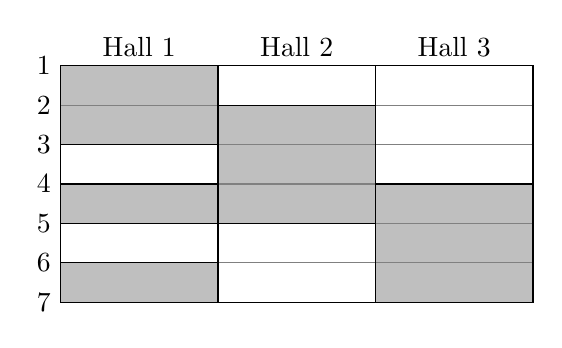
\begin{tikzpicture}
    \draw [white] (1,0) -- (1,3) node [text=black,above] {Hall 1}
                  (3,0) -- (3,3) node [text=black,above] {Hall 2}
                  (5,0) -- (5,3) node [text=black,above] {Hall 3};

    \draw [gray] (6,3.0) -- (0,3.0) node [text=black,left] {1}
                 (6,2.5) -- (0,2.5) node [text=black,left] {2}
                 (6,2.0) -- (0,2.0) node [text=black,left] {3}
                 (6,1.5) -- (0,1.5) node [text=black,left] {4}
                 (6,1.0) -- (0,1.0) node [text=black,left] {5}
                 (6,0.5) -- (0,0.5) node [text=black,left] {6}
                 (6,0.0) -- (0,0.0) node [text=black,left] {7};
    
    \draw [fill=none] (0,0) rectangle (2,3)
                      (2,0) rectangle (4,3)
                      (4,0) rectangle (6,3);

    \draw [fill=gray,fill opacity=0.5] (0,3.0) rectangle (2,2)
                                       (0,1.5) rectangle (2,1)
                                       (0,0.5) rectangle (2,0)
                                       (2,2.5) rectangle (4,1)
                                       (4,1.5) rectangle (6,0);
                      
\end{tikzpicture}
\end{center}
\caption{Scheduling Problem Solution}
\end{figure}